\chapter{Harmonogram realizacji projektu.}
\label{chap:harmonogram}

\section{Harmonogram realizacji projektu. - Diagram Gantta}
Harmonogram realizacji projektu jest kluczowym elementem planowania, który pozwala na efektywne zarządzanie czasem i zasobami. W projekcie dotyczącym systemu rezerwacji usług łowiska wędkarskiego, harmonogram został opracowany z uwzględnieniem wszystkich istotnych etapów, od analizy wymagań po testowanie i wdrożenie.
\begin {itemize}
    \item \textbf{Analiza wymagań:} Zbieranie i analiza wymagań funkcjonalnych i niefunkcjonalnych systemu.
    \item \textbf{Projektowanie architektury:} Opracowanie struktury projektu, w tym diagramów UML i schematu bazy danych.
    \item \textbf{Implementacja:} Programowanie poszczególnych komponentów systemu, takich jak warstwa dostępu do danych, logika biznesowa i interfejs użytkownika.
    \item \textbf{Testowanie i dokumentacja:} Przeprowadzenie testów jednostkowych i integracyjnych, a także przygotowanie dokumentacji użytkownika i technicznej.
\end{itemize}

\begin{figure}[H]
    \centering
    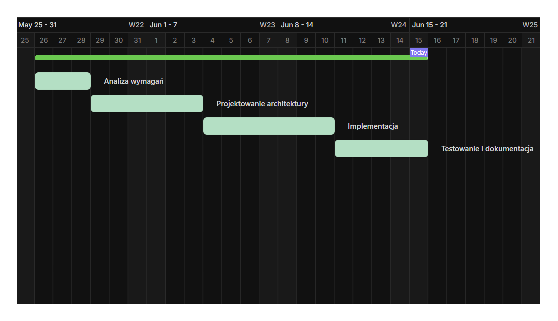
\includegraphics[width=\linewidth]{figures/gantt.eps}
    \caption{Harmonogram realizacji projektu (Diagram Gantta).}
    \label{fig:gantt_chart}
    \small{Źródło: Wygenerowano za pomocą https://clickup.com}
\end{figure}

\section{System kontroli wersji i repozytorium}
W projekcie zastosowano system kontroli wersji Git, który umożliwia śledzenie zmian w kodzie źródłowym, zarządzanie wersjami oraz współpracę zespołową. Git pozwala na tworzenie gałęzi (branch), co umożliwia równoległe prace nad różnymi funkcjonalnościami bez wpływu na główną linię rozwoju projektu.

Jako centralne, zdalne repozytorium kodu wykorzystano platformę GitHub. Cały projekt jest publicznie dostępny pod adresem:
\begin{center}
    \url{https://github.com/KamilKopczyk/Projekt_PO_JAVA_Kamil_Kopczyk_134927}
\end{center}




